\chapter{Quantitative methods for social research in the digital age}

Quantitative social scientists often attempt to understand the
behavior of political entities.  The digital age has brought to these
researchers a deluge of digital records---particularly in the form of
text.  This avalanche of data provides more information to these
scientists than they have had in the history of mankind.  Researchers
are now able to pore over digital copies of all legally binding
opinions written by United States Supreme Court Justices, or the text
of thousands of bills voted on by members of Congress.  Even these
numbers are dwarfed by the hundreds of thousands of newspaper articles
written about the international relations.  Unfortunately, this flood
of information obscures the very insights these researchers aim to
discover.  Researchers trying to make sense of these collections are
subject to the high costs of time spent poring over these collections
in search of the few key insights.

 % example questions: how to find phenomena in collections of text
 % how to 
% The goal of this thesis is to demonstrate that complex, meaningful patterns of
% information can be gleaned
% Society interacts with this information in
% a complicated dance: information affects what we do, and we create
% further information -- books, scientific papers, legislation, and
% tweets -- as a result.  Information influences everything we say,
% think, and do.
The goal of this thesis is to describe several new statistical models
to illustrate this -- and at the same time to provide tools for data
consumers, practitioners, and researchers\footnote{Throughout this
  work, I will refer to (data) consumers, practitioners, and
  researchers.  Consumers are those who use processed results from
  data analysis in some form but do not interact directly with the
  data itself (for example, consumers may be directors in governments
  or companies who make decisions based on these data).  Practitioners
  are those who apply existing methods for data analysis, possibly
  tweaking or combining these methods to answer specific questions
  (such as database engineers or lab assistants). Researchers are
  those who research entirely new methods for data analysis.  Note
  that a social scientist may be a researcher in his or her field but
  a practitioner in the field of data analysis.} to better
understanding society through collections of text documents.  I will
focus on three high-level research questions that dovetail off one
another to illustrate the flexibility and interpretability of latent
variable models in large-scale settings.

An implicit premise of this thesis is that these complex but
interpretable patterns are ubiquitous in collections of text
documents, and that these patterns be discovered automatically to
describe decisions and behavior of actors in these collections.  I will
ground this discussion with the development of several specific models
but take the position throughout this thesis that these methods draw
from a suite of common tools which can be used again and again to
construct models to address alternative questions.

\section*{The deluge of information and some statistical tools}

% The availability of observational social science data on a massive scale
Observational social science data -- including data about how
organizations and the Government work -- has become available on a
massive scale. The National Archives, which collects information from
over 500 federal agencies, has been digitizing its collection of
twelve \emph{billion} federal documents \citep{lazer:2009,
  national_archives:2012a,national_archives:2012b}.  The problem in
handling this data has moved from collecting the data to processing
and understanding it.

Fortunately for scholars, these data follow recurring patterns which
make statistical modeling possible. In this thesis, I will focus on
three specific patterns:

\paragraph{Text data.} This thesis will focus largely on text data.
Text data is the low-hanging fruit of most social science research
questions.  It is ubiquitous because it can---indeed, it must---be
easily created, digitized, and stored. One of the central themes of
this thesis is that text data serve as an observation of the story
underlying decisions and politics.

Just as text data is invaluable to researchers, the rate of growth of
these text collections is staggering.  A single newspaper like the
\emph{New York Times} publishes hundreds of thousands of articles each
decade.  Of the National Archive's collection, billions of its
documents are text
\citep{national_archives:2012a,national_archives:2012b}.  The rate of
growth for the World Wide Web is even more staggering.  As far back as
2008, the Internet was already growing at a rate of several billion
webpages per \emph{day} \citep{googleblog:2008}.

\paragraph{Time-series collections.}  Many datasets comprise
time-series observations.  Timestamps are one of the simplest types of
metadata to attach to digital collections because they are described
by a single scalar and because they are inexpensive and widely
available.  In addition, the dimension of time is especially
interesting to researchers because it is helpful in framing questions
about causation and prediction.

\paragraph{Dyadic observations.}  Dyadic relationships are one of the
simplest ways to represent more complicated phenomena in a collection
of data. In later chapters we will use spatial models to represent
interactions between lawmakers and bills (i.e., how congresspersons voted
on bills) and between countries (i.e., countries' sentiment
toward one another).  As we will show, the underlying representation
for these cases is very similar.

\subsection*{The role of statistical machine learning}

The deluge of information available to researchers means that
researchers cannot spend long looking over any document.  For example,
a researcher drawing conclusions about patterns governing the
relationships between pairs of countries, based on mentions of pairs
of countries in the \emph{New York Times}, would need to spend every
day of an entire year, twenty-four hours per day, two minutes per
mention, to code the 300,200 interactions per pair of countries.  A
\emph{computational} treatment is therefore necessary if researchers
intend to handle large collections of data.

In each of the models we will consider, the basic unit of analysis
lives in an extremely high-dimensional space.  For example, treating
text documents as bags of words still leaves the researcher with
thousands of dimensions, and lawmakers described by their votes are
still described by these thousands of
dimensions.% \cite{changrtl:2009}.
In addition to text, another recurring theme in this thesis is that
these high-dimensional observations can be described by much
lower-dimensional summaries without losing much of the relevant
information.

Computational approaches lend themselves to \emph{statistical}
representations of these data because they provide an explicit way to
formalize our assumptions.  Statistical representations are also
convenient because computers can be programmed to speak in this
language. Specifically, I will use probabilistic models to encode
these statistical assumptions.  I will frequently use the paradigm of
graphical models \citep{pearl:1985} to encode and describe our
assumptions.  Because these statistical methods provide directed
summaries, they can serve as optical lenses for researchers to analyze
entire collections of documents.  I illustrate this with a cartoon in
\myfig{person_data_lens}.  Statistical methods enable researchers to
describe arbitrarily complex transformations of data with arbitrarily
complex lenses, but I will demonstrate that a wide array of models can
be created by nesting and re-using modules across different
applications.

\begin{figure}
  \center
  \begin{tabular}{ccc}
    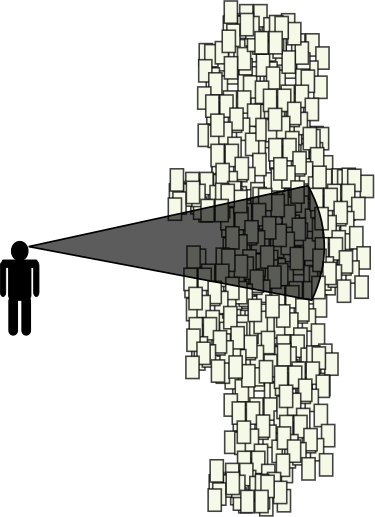
\includegraphics[width=0.3\textwidth,height=0.3\textwidth]{chapter_introduction/figures/person_data.pdf} &
    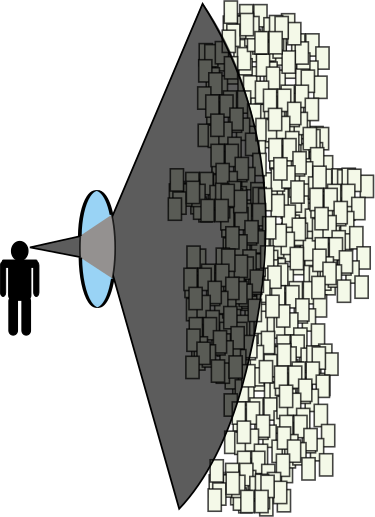
\includegraphics[width=0.3\textwidth,height=0.3\textwidth]{chapter_introduction/figures/person_data_lens.pdf} &
    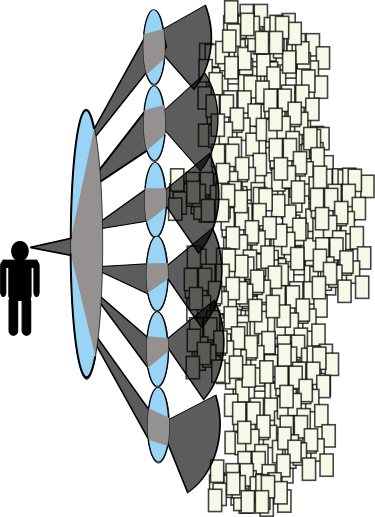
\includegraphics[width=0.3\textwidth,height=0.3\textwidth]{chapter_introduction/figures/person_data_lens2.pdf} \\
  \end{tabular}
  \caption{A cartoon illustration of the role of statistical models in
    large-scale data analysis.  Left: large data collections are too
    large to handle without special tools. Center, Right: statistical
    models serve as lenses which can be nested, adjusted, and
    custom-designed to glean latent structure from large or complex
    datasets.  Our statistical assumptions define the shape and
    optical characteristics of these lenses.}
  \label{fig:person_data_lens}
\end{figure}

% - Tools and abstractions for probabilistic inference

\section*{Organization}

By the end of this thesis, the reader should have a better
understanding of several new models available to social scientists.
Perhaps more importantly, the reader will be prepared to design his or
her own latent-variable model for similar applications.

To this end, I will provide a lower level of detail about
latent-variable models in the early chapters of this thesis when it is
appropriate to help the reader understand the material.  I provide
preliminary material in Chapter 2, outlining the statistical
``primitives'' that I will use as building blocks in later chapters.
These primitives include the basic statistical tools for working with
text data, time-series data, and dyadic data.  This chapter also
provides a high-level introduction to the tools we will use for
Bayesian inference.

\paragraph{Identifying influential documents.} In \mychap{influence} I
introduce a model for discovering important and influential documents
in a collection of documents which has grown over time.  In
collections of legal opinions, one of the most common questions posed
by jurists\footnote{In political science, the word ``jurist'' often
  refers to a judge, as opposed to a member of the public who votes on
  the outcome of a trial.} is, ``which legal opinions have set the
most precedent?''  This question plays a central role among
researchers and archivists in fields outside of law and even motivated
the algorithm behind Larry Page and Sergey Brin's PageRank algorithm,
which recursively measures the influence of Webpages, as measured by
the hyperlinks between Webpages
\citep{garfield:1992,brin:1998,garfield:2002}.  In many real-world
scenarios, however, explicit citations or hyperlinks are missing, and
researchers only see the most basic metadata: documents' timestamps.
I will validate this model on a set of several datasets, including
several collections of academic articles and a set of opinions written
by judges in the New York Appellate Courts system.

\paragraph{Inferring history from a collection of newspaper articles.}
In \mychap{foreign_relations} I outline a model to address the question
posed above, to better understand the relationships between countries
over time.  I will fit this to a collection of New York Times articles
and demonstrate that this method discovers a more sophisticated latent
story among documents, by developing a model of the relationships
between countries over time.  As with the method in Chapter 3, this
collection has only the text of these articles, which I augment with
external information.  In this chapter I also incorporate important
ideas from the field of dyadic spatial models, which can play a role
in modeling various social science phenomena.

% I will describe a method to discover
% which documents are influential on the development of a collection of
% text documents \emph{without} the use of metadata such as
% citations---where by an ``influential'' document I mean one that uses
% language which is adopted by others in the collection.

\paragraph{Inferring lawmakers' preferences.}

In \mychap{spatial_voting} I will extend existing spatial models to
better understand how Congressmen feel about different issues.  I
begin with a model which is able to predict how lawmakers will vote on
previously-unseen bills.  I will also describe a method for learning
lawmakers' issue preferences from their votes on different issues.

These models contrast with those in chapters 3 and 4 in that I ignore
documents' timestamps.  I will use some of the same ideas from Chapter
4, in which we we assume that pairs of items interact (in this case a
lawmaker and a bill), and that text documents attached to those
interactions can provide insight into the interaction.

\paragraph{Additional materials.}
In Appendix~\ref{chapter:stochastic_variational_optimization} I
discuss details of a new variational inference algorithm which is used
in \mychap{spatial_voting}.  This Appendix can be treated as a
stand-alone contribution of this thesis, making a quantitative rather
than a substantive contribution.  I provide additional supplementary
information for these chapters in
Appendix~\ref{chapter:supplementary_materials} as well as notes on
analysis of text datasets in Appendix~\ref{chapter:notes_text}.
